\section{Methods}
\label{sec:Methods}

\subsection{Manufacturing}

\subsubsection{Preparation of reagent}

All reagents were of analytic grade and were used as received from the suppliers without further  purification. Every chemical was bought from Sigma Aldrich, unless stated otherwise. 
Next for facilitation we introduced the formula making use of stoichiometry:

\begin{equation}
\label{eq:RedPrep}
    \frac{m'\cdot v\cdot M}{1000} = m(m',v,M)
\end{equation}


where $m'$ denotes the molecular weight of the reagent, $v$ the desired end-volume of the solution, $M$ the molar concentration and $m$ the needed amount of the substance with unit 'grams', assuming the chemical to be pure. (Example: We want to make 4ml (~$= v$) of solution with \ce{NaOAc} (~$m'_{\ce{NaOAc}}= 82.03 \frac{g}{mol}$) at a concentration of 0.25 M (~$= M$). We now know, that we need to dilute $m \approx 82mg$ \ce{NaOAc} in 4ml of solvent!) 

\paragraph{Gold solution}

We used Gold(III) chloride trihydrate, dissolved in 100 \% ethanol (EtOH). The concentration, unless stated otherwise, was 0.25M and was prepared using the formula (\ref{eq:RedPrep}).


\paragraph{Reduction agent solution}

From the identified reduction agents, the reagent was produced by taking the calculated amount and diluting it in Milli-Q \ce{H2O} until the concentration given was reached. Were the reduction agent was light-sensitive, we put aluminium-foil around the containing reservoir to decrease exposure.


\subsubsection[Sample Fabrication]{Sample Fabrication \label{subsec:SampleFab} \footnote{For more extensive protocol, see page \pageref{App:Protocols}}}


Define Experiment. We identified 5 independent variables that can be changed.


\begin{multicols}{2}
\begin{itemize}
    \item Gold concentration (\textit{c\textsubscript{gold}})
    \item Gold immersion time (\textit{t\textsubscript{gold}})
    \item Choice of reduction agent
    \item Reduction agent concentration (\textit{c\textsubscript{Red}})
    \item Reduction agent immersion time (\textit{t\textsubscript{Red}})
\end{itemize}
\end{multicols}




\paragraph{Initial Protocol}

\begin{enumerate}
	
	\item Immerse Fiber in Gold Salt Concentration with $c_{GoldConc}$ during $t_Gold$, then take out.

	\item Let the fiber dry for 30 minutes.
	
	\item After Drying, Immerse Fiber in Reduction Agent with $c_{Red}$ during $t_Red$, then take out.
	
	\item Let the fiber dry in petri dish for 1 hour, before proceeding with resistance measurement protocol.

    \end{enumerate}
    
    \begin{center}
        This marks the end of the fiber fabrication.
    \end{center}


\paragraph{Optimized Protocol} \hfill\newline

1. - 3. are identical to initial protocol.

\begin{enumerate}
\setcounter{enumi}{3}
	
	\item Let the fiber dry on glass slide for 1 hour, before proceeding with resistance measurement protocol.


\end{enumerate}
    
    \begin{center}
        This marks the end of the fiber fabrication.
    \end{center}

\subsection{Measurement}

\subsubsection{Preparation}
Prerequisites:
\begin{multicols}{2}
\begin{itemize}
    \item Sample with size $l$
    \item A small piece of paper
    \item 8 Pieces of Tape
    \item Silver Epoxy
    \item Derubberized Cable
\end{itemize}
\end{multicols}

Protocol:

\begin{enumerate}
	
    \item On piece of paper, put 1 piece of tape (Tape 1) on each side with distance $d < l$ from each other
    
    \item Now fix both ends of the sample gently without stretching (!) on Tape 1 with another piece of tape (Tape 2).
    
    \item Then, put free end of cable on end of sample, which is free and over Tape 1. Establish contact and fix cable with Tape 3.
    
    \item Put Silver Epoxy on sample-cable-interface to facilitate sample-cable-transmission. Bake at 80\textdegree C for 2h. After taking out the oven, put tape 4 perfectly aligned with the medial edge of Tape 1.
\end{enumerate}

    \begin{center}
    \myworries{
    TODO
    Refer to actual figure (Add label, fix picture organisation.)
    TODO}
    
See figure number \ref{fig:MeasPrep} in Appendix for visual description of resistance measurement preparation.
    \end{center}


\subsubsection{Resistance Measurements}

\begin{figure}[H]
    \centerline{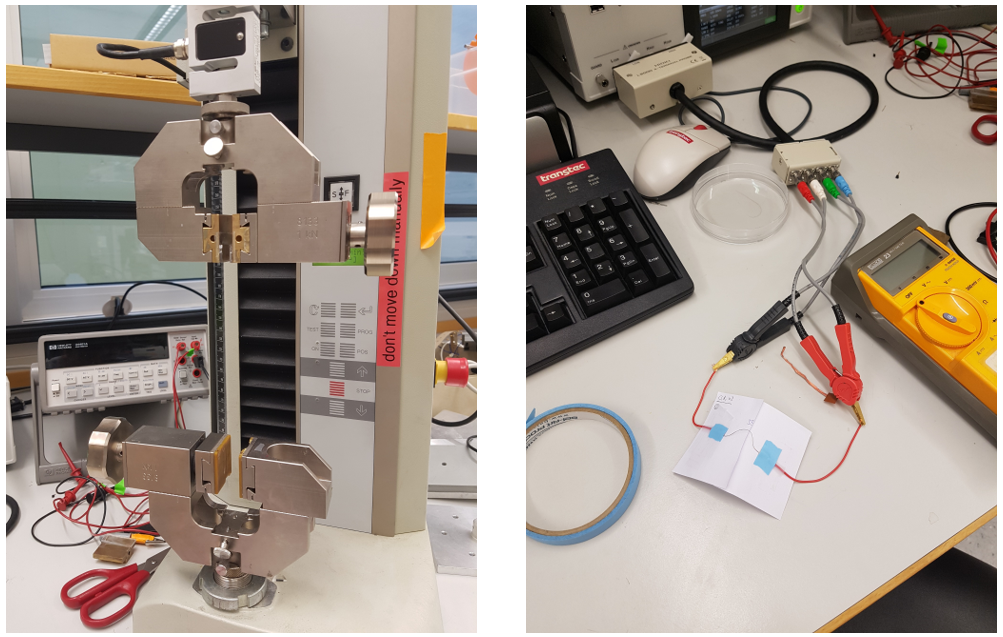
\includegraphics[scale=0.7]{./pic/MethodsResMeasurement.PNG}}
    \caption{Setup of Continuous Resistance Measurement}
    \label{fig:ContResMeas}
\end{figure}

Protocol:

\begin{enumerate}
	\item On piece of paper, put 1 piece of tape (Tape 1) on each side with distance $d < l$ from each other
	
	\item Now fix both ends of the sample gently without stretching (!) on Tape 1 with another piece of tape (Tape 2).
	
	\item Then, put free end of cable on end of sample, which is free and over Tape 1. Establish contact and fix cable with Tape 3.
	
	\item Put Silver Epoxy on sample-cable-interface to facilitate sample-cable-transmission. Bake at 80\textdegree C for 2h. After taking out the oven, put tape 4 perfectly aligned with the medial edge of Tape 1.
\end{enumerate}

